\documentclass[11pt,a4paper,uplatex,dvipdfmx]{ujarticle} 		% for uplatex
% \documentclass[11pt,a4j,dvipdfmx]{jarticle} 					% for platex
%=======================================
% form00_header.tex
%	General header for kakenhiLaTeX,  Moved over from form00_2010_header.tex.
%	2009-09-06 Taku Yamanaka (Osaka Univ.)
%==== General Version History ======================================
% 2006-05-30 Taku Yamanaka (Physics Dept., Osaka Univ.)
% 2006-06-02 V1.0
% 2006-06-14 V1.1 Use automatic calculation for cost tables.
% 2006-06-18 V1.2 Split user's contents and the format.
% 2006-06-20 V1.3 Reorganized user and format files
% 2006-06-25 V1.4 Readjusted all the table column widths with p{...}.
%				With \KLTabR and \KLTabRNum, now the items can be right-justified
%				in the cell defined by p{...}.
% 2006-06-26 V1.5 Use \newlength and \setlength, instead of \newcommand, to define positions.
% 2006-08-19 V1.6 Remade it for 2007 JFY version.
% 2006-09-05 V1.7 Added font declarations suggested by Hoshino@Meisei Univ.
% 2006-09-06 V1.8 Introduced usePDFform flag to switch the form file format.
% 2006-09-09 V1.9 Changed p.7, to allow different heights between years. (Thanks to Ytow.)
% 2006-09-11 V2.0 Added an option to show budget summary.
% 2006-09-13 V2.1 Added an option to show the group.
% 2006-09-14 V2.1.1 Cleaned up Kenkyush Chosho.
% 2006-09-21 V2.2 Generated under a new automatic development system.

% 2007-03-24 V3.0 Switched to a method using "picture" environment.

% 2007-08-14 V3.1 Switched to kakenhi3.sty.
% 2007-09-17 V3.2 Added \KLMaxYearCount
% 2008-03-08 V3.3 Remade it for 2009 JFY version\
% 2008-09-08 V3.4 Added \KLXf ... \KLXh.
% 2011-10-20 V5.0 Use kakenhi5.sty, to utilize array package in tabular environment.
% 2012-08-14 v5.1 Moved preamble and kakenhi5 into the current directory, instead of the parent directory.
% 2012-11-10 v6.0 Switched to kakenhi6.sty.
% 2015-08-26 v6.1 Added KLFirstPageIsLongPage flag.
% 2017-05-27 v7.0 Simplified for the new format.
% 2022-10-27 v7.1 Removed [dvipdfmx] from \usepackage{graphicx}.
%=======================================
% Dummy section and subsection commands.
% With these, some editors (such as TeXShop, etc.) can jump to the (sub)sections.
\newcommand{\dummy}{dummy}% 
\renewcommand{\section}[1]{\renewcommand{\dummy}{#1}}

\usepackage{calc}
\usepackage{geometry}                % See geometry.pdf to learn the layout options. There are lots.
\usepackage{graphicx}
\usepackage{color}
\usepackage{ifthen}
\usepackage{udline}
\usepackage{array}
\usepackage{longtable}
\usepackage{fancyhdr}
 % pieces
%==================================================
% kakenhi7.sty
%==================================================
% v1
% Minimum amount of macros for writing Kakenhi forms.
%
% 2005-10-24 Taku Yamanaka, Physics Dept. Osaka Univ.
%		taku@hep.sci.osaka-u.ac.jp
% 		Macros such as XYBC, etc. were imported from Kakenhi Macro at
% 		http://www.yukawa.kyoto-u.ac.jp/contents/researcher/kakenhi.html .
% 2006-06-04 Taku
%		Added macros to draw boxes if \DrawBox is in the source.
%		This is useful when designing the LaTeX forms.
% 2006-06-14 Taku
%		Added LaTeX macros to add costs 
%		(\KLResetGrandSum, \KLCostItem, \KLSum, \KLGrandSum).
%		Added a macro \Number to supply commas every 3 digits (imported from kkh.mac).
% 2006-06-25 Taku
%		Added \KLTabC, \KLTabR, \KLTabRNum to specify alignments in tables.
%		Please note that \phantom{...} is required for the column, 
%		or otherwise somehow p{...mm} is ignored.
% 2006-08-13 Taku
%		Added \KLItemNumUnitCost . This requires calc.sty.
% 2006-09-06 Taku
%		Added KLGrandTotalValue to add ALL the costs.
%		Also added \KLPrintGrandTotal to print the total on the console.
% 2006-09-09 Taku
%		Added macros to handle "efforts".
% 2006-09-10 Taku
%		Added \KLnewcounter to make series of counters.
%		Modified \KLResetGrandSum and \KLSum to add the sum for 
%		each category and year.
% 2006-09-11 Taku
%		Added \NumC to display LaTeX counter with commas.
% 2006-09-12 Taku
%		Added simple macros to make group table.
% 2006-09-23 Taku
%		Added the 'Fair License' notification.
% 2006-10-22 Taku
%		Initialize KLNumPeople to -1, so that the first header row will not be included in the count.
%====================================================
% v2
% 2007-03-24 Taku
%		Instead of using Kakenhi Macros to position items, 
%		switched to a new method using
%		"picture" environment.  The origin of the coordinate is set to 
%		the lower left corner of the paper.  The positions are given in "points", 
%		as can be read by gv. These methods were suggested by 
%		Tsutomu Sakurai at Saitama Univ..
% 2007-03-30 Taku
%		The sum of each category and year is made using 
%		macros \KLItemCost, etc., instead of \KLSum.  This is a step toward
%		automatically aligning category sums in the same year, in some forms.
% 2007-04-02 Taku
%		Added \KLBudgetMiniTabular, \KLMiniSum, etc. to handle
%		budget tables with multiple category columns.
% 2007-05-04 Taku
%		Added \multicolumnDottedLine .
%==================================================
% v3 
% 2007-08-14 Taku
%		Simplified page handling, by introducing \KLBeginSinglePage,
%		\KLPageRange, etc..
% 2007-09-01 Taku
%		Added a new command, \KLItemNumUnitCostLocation , 
%		and \KLAddCost to clean things up.
% 2007-09-06 Taku
%		Set \KLEven/OddLeft/RightEdge parameters in \KLWaterMark.
%		Without it, if \KLLeftEdge or \KLRightEdge is used inside watermark,
%		it generated a very obscure error message, which was hard to track down.
% 2007-09-09 Taku
%		Removed clearring \thiswatermark in \KLClearWaterMarks.
% 2007-09-12 Taku
%		Added \KLPriorityItemNumUnitCostTwo for Tokusui.
% 2007-09-14 Taku
%		Added \KLItemNumUnitCostTwo for tokutei_koubo.
% 2007-09-17 Taku
%		In \KLAddCost, costs are added only if it is within the defined year range.
% 2008-09-02 Taku
%		  Added \KLMonthPriorityItemNumUnitCostTwo for tokutei_keizoku.
% 2008-09-07 Taku
%		   Use \KLJFY to print year in budget tables.
% 2008-10-21 Taku
%			Added KLItemNumUnitCostInParen for shorei.
% 2009-09-03 Taku
%			Added \dottedLine .
%==================================================
% v4
% 2009-09-06 Taku
%			Added macros for partial typesetting.
% 2009-09-12 Taku
%			Added macros for showing coordinates and edges.
% 2009-09-13 Taku
%			Added macros to show boxes and minipage frames and their corner coordinates.
% 2010-03-04 Taku
%			Moved macros for calculating lengths and positions from form07_header.tex to here.
% 2010-04-11 Taku
%			Added \KLItemCostOne for jisedai, and necessary flags to print budget sums before 
%			the detailed budget table.
%==================================================
% v5
% 2011-10-20 Taku
%			By using array package within tabular environment, the following macros were simplified:
%			\KLTabC, \KLTabR, \KLBudgetMiniTabular, 
%			New Macros:
%			\KLCC, \KLCR
% 2011-10-24 Taku
%			Removed using \KLTabR from most of the budget tables.
% 2011-10-26 Taku
%			Added KLMyBudget.
%			Modified KLYearItemNumUnitCostTwo to just put the JFY if the second item is blank.  (For Kiban S)
% 2012-03-10 Taku
%			Changed the tabcolsep for \KLMyBudget to 0pt.
% 2012-08-14 Taku
%			Moved xxx_forms_pdf and _eps directories to under mother.
% 2012-09-09	Taku
%			Added \KLbibitem(B) and \KLcite(B).
% 2012-09-16	Taku
%			Added \KLOtherApplication, \KLOtherApplicationReasons, and \KLOtherFundReasons
%			for tokusui (and maybe for others in the future).
%==================================================
% v6
% 2012-11-10	Taku
% 			Modified \KLOtherApplicationReasons and \KLOtherFundReasons to make the tables compact.
%			These were in hook3.tex for the 2013 version.
%			Added \KLOtherApplicationDiff for many shumokus.
%			Removed \KLbibitemB and \KLciteB.
%			Changed \KLbibitem to use a dedicated column for numbering.
% 2012-11-11	Taku
%			Added \KLItemSetCostLocationInfo and \KLItemCostInfo.
% 2013-09-19	Taku
%			Added \KLOtherPD and \KLOtherPDShort to enter JSPS PD for other funds.
% 2013-10-02	Taku
%			Changed \KLbibItem, not to use a dedicated column for numbering, 
%			because otherwise the label defined in \label{...} cannot be used in @currentlabel.
% 2014-09-22	Taku
%			Added \KLCL for filling narrow tabular cells in English.  
%			(Suggested by Frank Bennett.)
% 2014-11-08	Taku
%			Added an instruction in \KLCheckPageLimit.
% 2015-08-23	Taku
%			Added NumCk to show numbers divided by 1000 (truncated).
% 2015-08-24	Taku
%			Introduced \KLLongPage and \KLSimpleLongPage to offer floating environment in 
%			single-page-frames.
%=====================================================
% v7
%	Frames are gone!  Simplify kakenhiLaTeX to benefit from 
%	the new style.
% 2017-05-03	Taku
%			Added \KLAnotherFund .
% 2017-05-27	Taku
%			Made \KLBeginSubject and \KLEndSubject to handle new 
%			mother file style.
% 2017-08-17 Taku
%	Added \KLItemCostNoYear and \KLEndBudgetNoYear for kokusai_kyoudou.
% 2017-08-19	Taku
%			Updated \KLBeginSubject and \KLEndSubject to handle 
%			various headers.
% 2017-08-20	Taku
%			\KLBeginSubject calls \KLFirstPageStyle and \KLDefaultPageStyle
%			which should be defined for each shumoku (or JSPS/MEXT).
%			This is to pass the subject name etc. to the header.
% 2017-08-27	Taku
%			Set section number in \KLBeginSubject.
% 2017-08-29	Taku
%			Moved over KLShumokuFirstPageStyle and KLShumokuDefaultPageStyle.
%			Added jsps-abs-p1-header, jps-abs-subject-header, and 
%			jsps-abs-default-header as arguments to \KLShumoku***Header.
% 2017-09-02	Taku
%			Added \KLBeginSubjectWithHeaderCommands for more flexible header style.
% 2017-09-03	Taku
%			Added \vspace*{-4mm} after \includegraphics in \KLBeginSubject*.
% 2017-09-05	Taku
%			Removed now-the-old commands.
% 2020-01-02	Taku
%			Added more numbers to \KLJint for gakuhen_a.
% 2020-01-15	Taku
%			Changed the horizontal position (none --> -3mm) 
%			and the width of the top boxes for headers (\linewidth --> 1.02\linewidth)
%			to reproduce the original boxes.  
%			This became necessary because the margins were set correctly in form02_header.tex.
% 2021-01-29	Taku
%			Set section counter and reset subsection counter only if the section # is given for
%			\KLBeginSubject and \KLBeginSubjectWithHeaderCommands .
% 2022-01-26	Taku
%			Changed the scale for the top boxes from 1.03 to 1.01, 
%			and \hspace from -3mm to -2mm.  (DC)
% 2022-02-23	Taku
%			Introduced \KLBoxOffset and \KLBoxScale for flexibility.
% 2022-03-20	Taku
%			Added '%' after \hspace{ } before incldegraphics.
% 2022-08-03	Taku
%			Use width=\KLBoxWidth, instead of \KLBoxScale*\linewidth which depents on
%			\linewidth.  (I should have noticed it earlier.)
% 2023-03-09	Taku
%			Added \vspace*{\KLBoxVOffset} to \KLBeginSubject.
% 2023-07-10	Taku
%			Added \includegraphics_full_width to place full-width 
%			instruction box images.
%			This is used also for \KLBeginSubject and 
%			\KLBeginSubjectWithHeaderCommands.  
%			\KLBoxOffset and \KLBoxWidth are not needed anymore.
%			Why didn't I think of it (-1in-\oddsidemargin) before??
%=====================================================

%=====================================================
% Macro to supply commas every 3 digits (up to 9 digits)
%	Imported from kkh.mac for Kakenhi Macro.
%=====================================================
%
\newif\ifNumWithCommas \NumWithCommastrue
\def\NumWithCommas{\NumWithCommastrue}
\def\NumWithoutCommas{\NumWithCommasfalse}
\newcount\Numa
\newcount\Numb
\def\Numempty{}%output blank if "-0" is given
\def\Number#1{\edef\Numpar{#1}\ifx\Numempty\Numpar\else%
\ifNumWithCommas\Numa=#1\relax
\ifnum\Numa>999999\divide\Numa by 1000000
\number\Numa,%
\multiply\Numa by -1000000\advance\Numa by #1\relax
\Numb=\Numa\divide\Numa by 1000
\ifnum\Numa<100 \ifnum\Numa<10 0\fi0\fi\number\Numa,%
\multiply\Numa by -1000\advance\Numa by \Numb
\ifnum\Numa<100 \ifnum\Numa<10 0\fi0\fi\number\Numa%
\else\ifnum\Numa>999\divide\Numa by 1000
\number\Numa,%
\multiply\Numa by -1000\advance\Numa by #1\relax
\ifnum\Numa<100 \ifnum\Numa<10 0\fi0\fi\number\Numa%
\else\number\Numa\fi\fi\else\number#1\fi\fi}

%======================================================
% Macro to display LaTeX counter with commas every 3 digits.
%======================================================
\newcommand{\NumC}[1]{\Number{\value{#1}}}

\newcounter{kyen}
\newcommand{\NumCk}[1]{%
	\setcounter{kyen}{\arabic{#1}/1000}
	\Number{\value{kyen}}
}

%======================================================
% Macros to align (right-justify, center) elements within a tabular cell
% whose width is defined by p{...}.
% 2006-06-25 Taku
% 	These are necessary, because the cell width should be given explicitly
% 	by p{...mm} to match the given table in a tabular environment.  
% 	One could allocate a width with \phantom{...},
% 	but it is a little tricky, since it depends on the font size.
%======================================================

%---------------------------------------------------------------------
% Center text within a tabular cell allocated by p{...}
%\newcommand{\KLTabC}[1]{\multicolumn{1}{c}{#1}}
\newcommand{\KLTabC}[1]{\centering\arraybackslash#1}
% This new method does not require a dummy table row to put them in correct columns.
%
% This should be used in tabular definition, as:
%	\begin{tabular}[t]{>{\KLCC}p{30pt}p{50pt}}
\newcommand{\KLCC}{\centering\arraybackslash}

%---------------------------------------------------------------------
% Right justify text within a tabular cell allocated  by p{...}
%\newcommand{\KLTabR}[1]{\multicolumn{1}{r@{\ }}{#1}}
\newcommand{\KLTabR}[1]{\raggedleft\arraybackslash#1}

% This should be used in tabular definition, as:
%	\begin{tabular}[t]{>{\KLCR}p{30pt}p{50pt}}
\newcommand{\KLCR}{\raggedleft\arraybackslash}%

%---------------------------------------------------------------------
% Right justify number (with comma every 3 digits) 
% within a tabular cell allocated by p{...}
\newcommand{\KLTabRNum}[1]{\KLTabR{\Number{#1}}}

%---------------------------------------------------------------------
% Left justify text within a tabular cell allocated by p{...}
% This should be used in tabular definition, as:
%	\begin{tabular}[t]{>{\KLCL}p{30pt}p{50pt}}
\newcommand{\KLCL}{\raggedright\arraybackslash}%

%=================================================
%  counter tools
%=================================================
\newcounter{KLtmp}

%------------------------------------------------------------------------------
% Makes a set of counters, with prefix #1, followed by 
% suffix ranging from 0 to #2 - 1.
% For example, \KLnewcounter{mine}{3} makes counters
% mine0, mine1, and mine2 .
%-------------------------------------------------------------------------------
\newcommand{\KLnewcounter}[2]{
	\setcounter{KLtmp}{0}
	
	\whiledo{\value{KLtmp} < #2}{
		\newcounter{#1\arabic{KLtmp}}
		\stepcounter{KLtmp}
	}
}

%------------------------------------------------------------------------------
% Dumps the contents of the counters.
%------------------------------------------------------------------------------
\newcommand{\KLdumpcounter}[2]{
	\setcounter{KLtmp}{0}
	
	\whiledo{\value{KLtmp} < #2}{
		#1\arabic{KLtmp} : \arabic{#1\arabic{KLtmp}}\\
		\stepcounter{KLtmp}
	}
}

%=======================================================
% LaTeX macros to add costs.
%	2006-06-14 Taku Yamanaka
%=======================================================
\newcounter{KLCost}				% to calculate cost = #units x unit cost
\newcounter{KLGrandTotalValue}		% for the grand total of all the categories in all years
\setcounter{KLGrandTotalValue}{0}

\newcommand{\KLCostCategory}{KLequipments}
\newcounter{KLYearCount}
\newcounter{KLPrintYear}

% Make counters for annual sums for each category-----------------------
\newcommand{\KLMaxYear}{8}
\KLnewcounter{KLequipments}{\KLMaxYear}
\KLnewcounter{KLexpendables}{\KLMaxYear}
\KLnewcounter{KLdomestic}{\KLMaxYear}
\KLnewcounter{KLforeign}{\KLMaxYear}
\KLnewcounter{KLtravel}{\KLMaxYear}
\KLnewcounter{KLgratitude}{\KLMaxYear}
\KLnewcounter{KLmisc}{\KLMaxYear}
\KLnewcounter{KLAnnualSum}{\KLMaxYear}

%------------------------------------------------
% Add up the given cost to category-year sum, category sum, year-sum, and total.
% 2007-09-01 Taku
% 2007-09-17 Taku: Add costs only if it is within the defined year range.
%------------------------------------------------
\newcommand{\KLAddCost}[1]{%
	\ifthenelse{\value{KLYearCount} > \value{KLMaxYearCount}}{%
		%pass
	}{%
		\addtocounter{\KLCostCategory0}{#1}%
		\addtocounter{\KLCostCategory\arabic{KLYearCount}}{#1}%
		\addtocounter{KLAnnualSum\arabic{KLYearCount}}{#1}%
		\addtocounter{KLAnnualSum0}{#1}%
		\ifthenelse{\equal{\KLCostCategory}{KLdomestic}}{%
			\addtocounter{KLtravel0}{#1}%
			\addtocounter{KLtravel\arabic{KLYearCount}}{#1}%
		}{}%
		\ifthenelse{\equal{\KLCostCategory}{KLforeign}}{%
			\addtocounter{KLtravel0}{#1}%
			\addtocounter{KLtravel\arabic{KLYearCount}}{#1}%
		}{}%
	}%
}


\newcommand{\KLClearWaterMarks}{%
	%--empty watermarks
	\watermark{}
%	\thiswatermark{}
	\rightwatermark{}
	\leftwatermark{}
}

\newcommand{\KLInput}[1]{%	The macros defined inside the file are only valid within the file.
	\begingroup
	\input{#1}
	\endgroup
}

%================================
% For 2017 new style without frames
%================================
\newcommand{\KLShumokuFirstPageStyle}[5]{%
%	Defines the header for the first page.
%	Called from \KLBeginSubject.
%--------------------------------
%	#1: page style name
%	#2: 様式
%	#3: 研究種目名
%	#4: 項目名
%	#5: sectionNo
%--------------------------------
	\ifthenelse{\equal{#1}{jsps-p1-header}}{%
		\JSPSVeryFirstPageStyle{#1}{#2}{#3}{#4}{#5}
	}{%
		\ifthenelse{\equal{#1}{jsps-abs-p1-header}}{%
			\JSPSVeryFirstPageStyle{#1}{#2}{#3 概要}{#4}{#5}
		}{%
            		\ifthenelse{\equal{#1}{jsps-subject-header}}{%
            			\JSPSFirstSubjectPageStyle{#1}{#2}{#3}{#4}{#5}
            		}{%
				\ifthenelse{\equal{#1}{jsps-abs-subject-header}}{%
            				\JSPSFirstSubjectPageStyle{#1}{#2}{#3 概要}{#4}{#5}
				}{%
                    			\thispagestyle{#1}
				}
            		}
		}
	}
}

\newcommand{\KLShumokuDefaultPageStyle}[5]{%
%	Defines the default header.
%	Called from \KLBeginSubject.
%--------------------------------
%	#1: page style name
%	#2: 様式
%	#3: 研究種目名
%	#4: 項目名
%	#5: sectionNo
%--------------------------------
	\ifthenelse{\equal{#1}{jsps-default-header}}{%
		\JSPSDefaultPageStyle{#1}{#2}{#3}{#4}{#5}
	}{%
		\ifthenelse{\equal{#1}{jsps-abs-default-header}}{%
			\JSPSDefaultPageStyle{#1}{#2}{#3 概要}{#4}{#5}
		}{%
            		\pagestyle{#1}
		}
	}
}

\newcommand{\KLSubjectName}{}
\newcommand{\KLSubjectMaxPages}{}
\newcommand{\KLSubjectEndPage}{}
\newcounter{KLSubjectEndPage}
\setcounter{KLSubjectEndPage}{0}

\newcommand{\KLSubjectCheckNPages}{%
%	\arabic{page}, \arabic{KLSubjectEndPage}\\
	\ifthenelse{\value{page}>\value{KLSubjectEndPage}}{
		{\LARGE「\KLSubjectName」は \KLSubjectMaxPages\ ページ以内で書いてください。}
		\clearpage
	}{%
	}
}

\newcommand{\KLSubjectAdvancePages}{%
	\renewcommand{\KLSubjectEndPage}{\value{KLSubjectEndPage}}
	\ifthenelse{\value{page}<\KLSubjectEndPage}{%
		\phantom{x}\clearpage
	}{}
	% Advance page if necessary
	\ifthenelse{\value{page}<\KLSubjectEndPage}{%
		\phantom{x}\clearpage
	}{}
	% Advance page if necessary
	\ifthenelse{\value{page}<\KLSubjectEndPage}{%
		\phantom{x}\clearpage
	}{}
	% Advance page if necessary
	\ifthenelse{\value{page}<\KLSubjectEndPage}{%
		\phantom{x}\clearpage
	}{}
	% Advance page if necessary
	\ifthenelse{\value{page}<\KLSubjectEndPage}{%
		\phantom{x}\clearpage
	}{}
}	

\newcommand{\KLJInt}[1]{%
% Returns full-width numerical character.
	\ifthenelse{\equal{#1}{1}}{1}{%
	\ifthenelse{\equal{#1}{2}}{2}{%
	\ifthenelse{\equal{#1}{3}}{3}{%
	\ifthenelse{\equal{#1}{4}}{4}{%
	\ifthenelse{\equal{#1}{5}}{5}{%
	\ifthenelse{\equal{#1}{6}}{6}{%
	\ifthenelse{\equal{#1}{7}}{7}{%
	\ifthenelse{\equal{#1}{8}}{8}{%
	\ifthenelse{\equal{#1}{9}}{9}{%
	\ifthenelse{\equal{#1}{10}}{10}{%
	\ifthenelse{\equal{#1}{11}}{11}{%
	\ifthenelse{\equal{#1}{12}}{12}{%
	\ifthenelse{\equal{#1}{13}}{13}{%
	\ifthenelse{\equal{#1}{14}}{14}{%
	\ifthenelse{\equal{#1}{15}}{15}{%
	\ifthenelse{\equal{#1}{16}}{16}{%
	\ifthenelse{\equal{#1}{17}}{17}{%
	#1}}}}}}}}}}}}}}}}}%
}

\newcommand{\includegraphicsFullWidth}[1]{%
	\noindent%
	\hspace{-1in-\oddsidemargin}%
	\includegraphics[width=\paperwidth]{#1}%
}

\newcommand{\KLBeginSubject}[8]{%
%----------------------------------------------------
%	#1: subjectNo
%	#2: sectionNo
%	#3: sectionJ
%	#4: maxPages
%	#5: pageLengthStyle ('V' for variable, 'F' for fixed)
%	#6: pageCounter (set page counter to this value if the argument exists.
%	#7: subjectFirstPageHeader (header for the first page)
%	#8: defaultPageHeader
%----------------------------------------------------
	\ifthenelse{\equal{#2}{}}{%
	}{%
	    	\setcounter{section}{#2}
	    	\setcounter{subsection}{0}
	}
	\setcounter{subsubsection}{0}
	\renewcommand{\KLSubjectName}{#3}
	\renewcommand{\KLSubjectMaxPages}{#4}
	
	\ifthenelse{\equal{#6}{}}{%
	}{%
		\setcounter{page}{#6}
	}
	
	\setcounter{KLSubjectEndPage}{\value{page}}
	\addtocounter{KLSubjectEndPage}{#4}
	
	\ifthenelse{\equal{#7}{}}{%
		% pass
	}{%
		\KLShumokuFirstPageStyle{#7}{\様式}{\研究種目header}{#3}{#2}
	}
	
	\ifthenelse{\equal{#8}{}}{%
		% pass
	}{%
		\KLShumokuDefaultPageStyle{#8}{\様式}{\研究種目header}{#3}{#2}
	}
	
	\vspace*{\KLBoxVOffset}%
%	\noindent
%	\hspace{\KLBoxOffset}%
%	\includegraphics[width=\KLBoxScale\linewidth]{subject_headers/\KLYoshiki_#1.pdf}\\
	\includegraphicsFullWidth{subject_headers/\KLYoshiki_#1.pdf}
	\vspace*{-4mm}
}

\newcommand{\KLNullHeader}[5]{}
% Dummy command for No header.
% This was introduced to avoid error caused in statement \ifthenelse{\equal{#8}{}} .

\newcommand{\KLBeginSubjectWithHeaderCommands}[8]{%
%----------------------------------------------------
%	#1: subjectNo
%	#2: sectionNo
%	#3: sectionJ
%	#4: maxPages
%	#5: pageLengthStyle ('V' for variable, 'F' for fixed)
%	#6: pageCounter (set page counter to this value if the argument exists.
%	#7: LaTeX command for subjectFirstPageHeader (header for the first page)
%	#8: LaTeX command for defaultPageHeader
%----------------------------------------------------
	\ifthenelse{\equal{#2}{}}{%
	}{%
		\setcounter{section}{#2}
		\setcounter{subsection}{0}
	}
	\setcounter{subsubsection}{0}
	\renewcommand{\KLSubjectName}{#3}
	\renewcommand{\KLSubjectMaxPages}{#4}
	
	\ifthenelse{\equal{#6}{}}{%
	}{%
		\setcounter{page}{#6}
	}

	\setcounter{KLSubjectEndPage}{\value{page}}
	\addtocounter{KLSubjectEndPage}{#4}
	
	#7{#7}{\様式}{\研究種目header}{#3}{#2}
	#8{#8}{\様式}{\研究種目header}{#3}{#2}
	
	\vspace*{\KLBoxVOffset}%
%	\noindent
%	\hspace{\KLBoxOffset}%
%	\includegraphics[width=\KLBoxWidth]{subject_headers/\KLYoshiki_#1.pdf}\\
	\includegraphicsFullWidth{subject_headers/\KLYoshiki_#1.pdf}
	\vspace*{-4mm}
}

\newcommand{\KLEndSubject}[1]{%
%	#1: pageLengthStyle ('V' for variable, 'F' for fixed)
		\clearpage % This should be done to update page counter for checking.
		\KLSubjectCheckNPages
		\ifthenelse{\equal{#1}{F}}{%
			\KLSubjectAdvancePages
		}{%
		}
}

%==================================================
% Miscellaneous macros
%==================================================

%----------------------------------------------------------------------
% Draw dotted lines across a multiple column table
%----------------------------------------------------------------------
\newcommand{\multicolumnDottedLine}[1]{%
%	\multicolumn{#1}{@{\hspace{-2mm}}c}{\dotfill}\\%
	\multicolumn{#1}{@{}c}{\dotfill}\\%
}

\newcommand{\dottedLine}{%
	\\\noindent
	\dotfill\\
}

%----------------------------------------------------------------------
% Solid line
%----------------------------------------------------------------------
\newlength{\KLLineLength}
\newcommand{\solidLine}[1]{
%----------- keep an empty line between here and \noindent so that it works after normal text and list.

	\noindent
	\hspace*{-10pt}
	\rule[10pt]{\textwidth}{#1}% #1 = 0.5pt, ....
	\vspace*{-10pt}
}

\newcommand{\KLLine}{%
	\solidLine{1pt}
}

%----------------------------------------------------------------------
% publication list (Thanks to Tetsuo Iwakuma [bulletin board #876])
%----------------------------------------------------------------------
\newcounter{KLBibCounter}

\makeatletter	
	\newcommand{\KLbibitem}{%
		\stepcounter{KLBibCounter}%
		\let \@currentlabel \theKLBibCounter
		\arabic{KLBibCounter}. %
	}
\makeatother

\newcommand{\KLcite}[1]{[\ref{#1}]}

%==================================================
%Fair License

%<Copyright Information>

%Usage of the works is permitted provided that this
%instrument is retained with the works, so that any entity
%that uses the works is notified of this instrument.

%DISCLAIMER: THE WORKS ARE WITHOUT WARRANTY.

%[2004, Fair License: rhid.com/fair]
%==================================================
% You may edit/modify this package at your own risk.
% If there are important fixes or changes that you think should be 
% reflected in the standard distribution, please notify:
%	taku@hep.sci.osaka-u.ac.jp  .
%==================================================
 % pieces
% form01_header.tex
% 2017-05-28 Split from form00_header.tex to move \input{kakenhiLaTeX7.sty} to mother_1.tex.
% 2010-01-15 Adjusted margins.
% 2022-02-23 Introduced \KLBoxOffset and \KLBoxScale.
% 2022-07-25 Introduced \KLBoxVOffset.
% ===== Parameters for KL (Kakenhi LaTeX) ========================
%%\geometry{noheadfoot,scale=1}  %scale=1 resets margins to 0
\setlength{\unitlength}{1pt}

\newlength{\KLCella}
\newlength{\KLCellb}
\newlength{\KLCellc}
\newlength{\KLCelld}
\newlength{\KLCelle}
\newlength{\KLCellf}

\newcounter{KLMaxYearCount}	% # of years for the proposal
\newcommand{\KLCLLang}{}	% language-dependent left-justification in tabular

% ===== format and header =========
% 2020-01-15: Reset it to match the margins (25 mm on sides, 20 mm on top and bottom). 
% A4: 294 mm x 210 mm.  
% LaTeX's default margin is 1 inch = 25.4 mm.
\setlength{\oddsidemargin}{-1pt}	% (25.0 - 25.4) / 25.4 * 72 pt/inch = -1 pt
\setlength{\evensidemargin}{-1pt}
\setlength{\textwidth}{453pt}		% (210 - 25*2) / 25.4 * 72 = 453 pt
\setlength{\topmargin}{-61pt}	% This and \headheight determine the actual top margin
\setlength{\textheight}{254mm}		% (294 - 20*2) = 254 mm

\setlength{\headheight}{48pt}
\setlength{\headsep}{3pt}

\cfoot{}
\renewcommand{\headrulewidth}{0pt}

\newcommand{\KLBoxVOffset}{-12pt}
\newcommand{\KLBoxOffset}{-25mm}
\newcommand{\KLBoxScale}{1.313}
\newcommand{\KLBoxWidth}{210mm}

\pagestyle{empty}
% ==== other applications table =========
\newcommand{\KLTableHeaderFont}{\fontsize{8.2}{11}\selectfont}
\newcommand{\KLTableHeaderSmallFont}{\fontsize{7.5}{10}\selectfont}
\newcommand{\KLTableHeaderSmallerFont}{\fontsize{7}{10}\selectfont}

 % pieces
% ===== Global year-dependent definitions for the Kakenhi form ===========
% 基本情報
\newcommand{\研究開始年度}{2024}
\newcommand{\研究開始元号年度}{06}	%令和

\newcommand{\一年目西暦}{2024}
\newcommand{\二年目西暦}{2025}
\newcommand{\三年目西暦}{2026}
\newcommand{\四年目西暦}{2027}
\newcommand{\五年目西暦}{2028}
\newcommand{\六年目西暦}{2029}

\newcommand{\一年目}{6}
\newcommand{\二年目}{7}
\newcommand{\三年目}{8}
\newcommand{\四年目}{9}
\newcommand{\五年目}{10}
\newcommand{\六年目}{11}

\newcommand{\一年目J}{6}
\newcommand{\二年目J}{7}
\newcommand{\三年目J}{8}
\newcommand{\四年目J}{9}
\newcommand{\五年目J}{10}
\newcommand{\六年目J}{11}


 % pieces
% hook3: after including packages ===================
 % pieces
%#Name: kiban_c
% form04_jsps_headers.tex
% 2017-08-20 Taku
% 2017-08-29 Taku
%			Added a check against jsps-abs-p1-header.
% 2017-09-02 Taku
%			Added sectionNo to the commands to make them compatible with 
%			\KLBeginSubjectWithHeaderCommands.
%			Use \KLJInt.
% 2018-09-01 Taku
%			Adjusted the heights of the headers by inserting \vspace{-3pt} and \rule.
%
\newcommand{\headerfont}{\fontsize{11}{11}\selectfont}
% ===== Headers =====================================
\newcommand{\JSPSVeryFirstPageStyle}[5]{%
%	Defines the header for the very first page of the form.
%	Called from \KLShumokuFirstPageStyle in form04_***.
%--------------------------------
%	#1: page style name
%	#2: 様式
%	#3: 研究種目名
%	#4: 項目名
%	#5: sectionNo
%--------------------------------
	\fancypagestyle{JSPSVeryFirstPageStyle}{% The name is not taken from #1, because 
		\fancyhf{}
		\fancyhead[L]{\hspace{-37pt}\headerfont#2\ 研究計画調書(添付ファイル項目)\\
				\rule{0pt}{18pt}\\}
%				\rule{0pt}{0pt}\\}
		\fancyhead[R]{\headerfont\textbf{#3\ \KLJInt{\thepage}}\vspace{-5pt}\\
			\rule{0pt}{0pt}\\}
%		\fancyhead[R]{\headerfont\textbf{#3\ \KLJInt{\thepage}\\}}
	}
	\thispagestyle{JSPSVeryFirstPageStyle}
}

\newcommand{\JSPSFirstSubjectPageStyle}[5]{%
%	Defines the header for the first page for the subject.
%	Called from \KLShumokuFirstPageStyle in form04_***.
%--------------------------------
%	#1: page style name
%	#2: 様式
%	#3: 研究種目名
%	#4: 項目名
%	#5: sectionNo
%--------------------------------
	\fancypagestyle{JSPSFirstSubjectPageStyle}{%
		\fancyhf{}
		\fancyhead[R]{\headerfont\textbf{#3\ \KLJInt{\thepage}}\vspace{-5pt}\\
			\rule{0pt}{0pt}\\}
%		\fancyhead[R]{\headerfont\textbf{#3\ \KLJInt{\thepage}\\}}
	}
	\thispagestyle{JSPSFirstSubjectPageStyle}
}

\newcommand{\JSPSDefaultPageStyle}[5]{%
%	Defines the default header for the subject.
%	Called from \KLShumokuDefaultPageStyle in form04_***.
%--------------------------------
%	#1: page style name
%	#2: 様式
%	#3: 研究種目名
%	#4: 項目名
%	#5: sectionNo
%--------------------------------
	\fancypagestyle{JSPSDefaultPageStyle}{%
		\fancyhf{}
		\fancyhead[L]{\headerfont\textbf{【#4(つづき)\ 】}\vspace{-7pt}\\}
		\fancyhead[R]{\headerfont\textbf{#3\ \KLJInt{\thepage}}\vspace{-5pt}\\
			\rule{0pt}{0pt}\\}
%		\fancyhead[R]{\headerfont\textbf{#3\ \KLJInt{\thepage}\\}}	
        }
        \pagestyle{JSPSDefaultPageStyle}
}

 % pieces
% form04_kiban_c_header.tex

% ===== Global definitions for the Kakenhi form ======================
% 基本情報
\newcommand{\様式}{様式S−14}
\newcommand{\研究種目}{基盤研究}
\newcommand{\研究種目後半}{(一般)}
\newcommand{\研究種別}{(C)}
\newcommand{\研究種目header}{\研究種目\研究種別\研究種目後半}

\newcommand{\KLMainFile}{kiban\_c.tex}
\newcommand{\KLYoshiki}{kiban_c_header}

%==========================================================
 % pieces
% ===== Global definitions for the Kakenhi form ======================
% 基本情報
%
%------ 研究課題名  -------------------------------------------
\newcommand{\研究課題名}{伝統的な木造土塗り壁の復元力に及ぼす軸組の影響に関する実験研究}

%----- 研究機関名と研究代表者の氏名-----------------------
\newcommand{\研究機関名}{公立鳥取環境大学}
\newcommand{\研究代表者氏名}{中治弘行}
\newcommand{\me}{{Hiroyuki Nakaji}}
\newcommand{\私}{{\研究代表者氏名}}

%---- 研究期間の最終年度 ----------------
\newcommand{\研究期間の最終元号年度}{8}  %令和で、半角数字のみ
%========================================

%inst_general_images.tex
\newcommand{\JSPSInstructions}{%
	\textcolor{red}{(\texttt{\textbackslash JSPSInstructions}をコメントアウトしてください。)}\\
	\includegraphicsFullWidth{subject_headers/inst_general.pdf}
}

\newcommand{\PapersInstructions}{%
	\textcolor{red}{(\texttt{\textbackslash PapersInstructions}をコメントアウトしてください。)}\\
	\includegraphicsFullWidth{subject_headers/inst_papers.pdf}
}
 % pieces
% user07_header
% ===== my favorite packages ====================================
% ここに、自分の使いたいパッケージを宣言して下さい。
\usepackage{wrapfig}
%\usepackage{amssymb}
%\usepackage{mb}
%\DeclareGraphicsRule{.tif}{png}{.png}{`convert #1 `dirname #1`/`basename #1 .tif`.png}
\usepackage{lineno}
\usepackage{graphicx}
\usepackage{ulem}
\usepackage{newcent}
\usepackage{url}
\urlstyle{same}

\makeatletter
\newcommand{\figcaption}[1]{\def\@captype{figure}\caption{#1}}
\newcommand{\tblcaption}[1]{\def\@captype{table}\caption{#1}}
\makeatother

% ===== my personal definitions ==================================
% ここに、自分のよく使う記号などを定義して下さい。
\newcommand{\klpionn}{K_L \to \pi^0 \nu \overline{\nu}}
\newcommand{\kppipnn}{K^+ \to \pi^+ \nu \overline{\nu}}

% ----- 業績リスト用 -------------
\newcommand{\paper}[6]{%
	% paper{title}{authors}{journal}{vol}{pages}{year}
	\item ``#1'', #2, #3 {\bf #4}, #5 (#6).			% お好みに合わせて変えてください。
}

\newcommand{\etal}{\textit{et al.\ }}
\newcommand{\ca}[1]{*#1}	% corresponding author;   \ca{\yukawa}  みたいにして使う
\newcommand{\invitedtalk}{招待講演}

\newcommand{\yukawa}{H.~Yukawa}					% no underline
%\newcommand{\yukawa}{\underline{\underline{H.~Yukawa}}}	% with 2 underlines
\newcommand{\tomonaga}{S.~Tomonaga}

\newcommand{\prl}{Phys.\ Rev.\ Lett.\ }		% よく使う雑誌も定義すると楽

% ===== 欄外メモ ==================
\newcommand{\memo}[1]{\marginpar{#1}}
%\renewcommand{\memo}[1]{}	% 全てのメモを表示させないようにするには、行頭の"%"を消す

% hook5 : right before \begin{document} ==============
 % pieces

\begin{document}
% hook7 : right after \begin{document} ==============
 % pieces
%#Split: 01_purpose_plan  
%#PieceName: p01_purpose_plan
% p01_purpose_plan_00.tex
\KLBeginSubject{01}{1}{1 研究目的、研究方法など}{4}{F}{}{jsps-p1-header}{jsps-default-header}

\section{1 研究目的、研究方法など}
%    <<最大 4ページ>>

%s02_purpose_plan_with_abstract_3p
% \JSPSInstructions		% <-- 留意事項。これは消すか、コメントアウトしてください。
\noindent
\textbf{(概要)}\\
%begin 研究目的及び研究計画の概要空行付き ====================
\hspace{1zw}伝統的構法木造建物の耐震診断及び耐震設計法については、2019年6
月に設計者向けのマニュアルが発行された。伝統的構法木造建物の主要な耐震要素
である土塗り壁の復元力特性は、検証実験結果に基づいて木造軸組の復元力$Q_f$
とその内側にある「土壁パネル」の復元力$Q_w$の和で得られるとされている。
$Q_f$と$Q_w$を分けて考え、あとで足し合わせる方法であり、実用面では簡便と言
える。
本研究では、特に$Q_w$の算定について、様々なサイズの土壁パネルの面内
せん断加力実験方法を開発し、計算方法の妥当性を再検証することを目的とする。

適切な試験体形状を提案するため、まず軸組接合部(仕口)の回転抵抗が0となるよ
う、仕口をピン接合として、軸組の木材同士の接触を避けるようにすきまを空ける
ことを考える。その方法により実大実験を行って、学術的にさらに充実したマニュ
アルへと発展させ、伝統的構法木造建物の安全・安心な保存活用と合わせ、新たな
建設と利用にも繋げていくことを目指す。
\vspace*{0zw}	% (概要)と(本文)の間が10行程度になるよう、必要に応じて値を調整してください。	
%end 研究目的及び研究計画の概要空行付き ====================

\noindent
\rule{\linewidth}{1pt}\\
\noindent
\textbf{(本文)}
%begin 研究目的と研究計画 ====================
\vspace{-1em}

\paragraph{(1) 本研究の学術的背景、研究課題の核心をなす学術的「問い」}
\mbox{}\vspace{-\baselineskip}
\paragraph{(1)-1 学術的背景}
\mbox{}\par

日本は地震国であるため、地震に対する備えが極めて重要であることはあらためて
言うまでもない。また、日本では木材や土、稲藁等の自然素材による建築が歴史的
にも長く用いられており、日本の気候風土にも適応した木造文化とも言えよう。日
本の伝統的な木造建物の耐震性能を確保することは、鳥取県内にも多く存在する文
化財等の古いものを残すためばかりではなく、伝統的な大工技術継承の観点から、
今後も新築ができるようにしていくことが大切である。

伝統的構法に限らず、木造(木質構造)建物の耐震性能や火災に対する安全性につい
ては、継続的にこれを調査・研究して、安心感を高める必要がある。
% 有史以来の度重なる地震被害はもとより、先の大戦中には空襲の被害を減ら
% すためとして、当時は耐火的とは言いがたい木造建築を減らすことも提案されてい
% た\cite{tanabe1933}。また、日本建築学会が、(1959年)9月の伊勢湾台風で受けた
% 甚大な被害にかんがみ、建築物の火災、風水害の防止を目的として、特に危険の著
% しい地域に対する建築制限のひとつとして「木造禁止」を提起し
% た\cite{aij-sengen1959} (2011年の日本建築学会大会でのパネルディスカッション
% で再考された\cite{mokuzousaiko2011})ことの影響もあったのだろう、
1960年代以降の一時期、日本建築学会での木造建物に関する研究は激減していた
が、1995年兵庫県南部地震による阪神・淡路大震災での木造住宅の大被
害\cite{aij1995}をふまえ、木質構造建物の耐震性能に関する研究は再びその数を
増やし、伝統的な土塗り壁に関する研究も見直されはじめ
た\cite{tuchikabe1999,murakami2005}。

木質構造の構造計算においては、建築基準法施行令第46条で規定される「構造耐力
上必要な軸組等」をチェックするいわゆる壁量計算の他、許容応力度設計と限界耐
力計算が用いられる。本研究でいう伝統的構法では、許容応力度設計と限界耐力計
算が適しており、限界耐力計算を用いれば建物の振動特性を考慮して地震応答を予
測できる利点がある。一方で、限界耐力計算では構造物の復元力特性の評価がとて
も重要であるが、伝統的構法を含め、木質構造の耐震性能評価では、この難易度が
壁量計算に比べてはるかに高いという問題があるため、理論的に明解で、実験でも
確認され、実用上簡便である手法の構築が求められてきた。

1999年から2002年までの3年間、日本建築学会に「木構造と木造文化の再構築」特別
研究委員会が設置され\cite{sympo2001}、2000年鳥取県西部地
震\cite{kitahara2002}では倒壊のような大被害の少なかった伝統的構法木造建物の
耐震性能もまた、見直されるようになった。その後、2008年から2012年まで5年間、
「伝統的構法の設計法作成及び性能検証実験」検討委員会\cite{kentouiinkai} (以
下、検討委員会)により、伝統的構法木造建物の耐震診断ならびに耐震設計法に関す
る提案がなされた\cite{kentouiinkai2012}。

この提案\cite{kentouiinkai2012}をふまえ、伝統的構法木造建物の耐震診断及び耐
震設計法について、2019年6月に設計者向けのマニュアル\cite{manual2019}が発行
され、構造計算適合性判定等手続き上の煩雑さは残るものの、必要な計算手法が明
記され、実務面では対応できるようになってきた。

\paragraph{(1)-2 研究課題の核心をなす学術的「問い」}
\mbox{}\par

% しかしながら、理論的には実用上の大きな問題がない程度に確かだが検証実験
% による裏付けが不足しているために理論的・実験的に研究を継続するべき事柄も残
% されている。例えば、伝統的構法木造建物の主要な耐震要素である土塗り壁の復元
% 力特性について、これまでの実大実験結果(その一部は応募者による)には矛盾しな
% い理論的な計算方法が示されているものの、実際の建物での使用が想定されるあら
% ゆるケースに対応できているとはまだ言いがたい状況である。特に、
土塗り壁の耐震性能(復元力特性、耐力と変形性能)を評価するには、それを構成す
る木造軸組の力学特性ならびに小舞下地や壁土の力学特性とその付着状況等を樹種
や壁土の性状に基づいて構造力学的に考える必要がある。しかし、実大実験結果と
材料レベルからの積み重ねによる評価をすっきりと結びつけることができる手法の
確立には至っていない。本研究では、実大実験要素を細分化し、材料特性→実大の
方向性を見据えつつ、実大実験→材料特性の方向で、材料試験と実物による実大実
験の間をつなぐことを目指している。

土塗り壁は伝統的構法木造建物において主要な耐震要素であるため、\textbf{理論
  的な考え方を実大実験で適切に裏付け、その耐震性能、復元力特性をより正しく
  予測できるようにしていくことは極めて重要}である。そして、実用的なマニュア
ルを一層充実させ、伝統的な建物の設計、利用に関わる人たちが安心できるように
していく必要がある。
% 新型コロナウィルス感染状況の影響で当面の実現は困難だが、
% 公開実験等を通して、このような研究による成果を様々な人たちに学んでもらう機
% 会を拡げることも重要である。

\paragraph{(2) 本研究の目的および学術的独自性と創造性}
\mbox{}\par

木造建物で耐震要素として用いられるいわゆる{「耐力壁」}では、軸組と面材パネ
ル要素を合わせた復元力特性を接合具の特性から構造力学的に評価する手法が提案
されているが、これらを一体として復元力特性(力と変形の関係)や耐震性能を議論
されることが多い\cite{kyoyououryoku2017}。伝統的構法木造建物で主要な耐震要
素である土塗り壁の復元力特性は、現時点では材料特性に基づく手法ではなく実大
実験結果に基づいて、木造軸組の復元力$Q_f$とその内側にある\textbf{「土壁パネ
  ル」}の復元力$Q_w$ (貫下地の復元力を含む) の重ね合わせで得られると仮定されてい
る。図\ref{fig:1}と図\ref{fig:2}にその考え方の概要を示す。
% $Q_f$と$Q_w$を分けて考え、あとで足し合わせ
% る方法である。
マニュアル\cite{manual2019}では、様々な土塗り壁の実大実験結果(一部は検討委員会の成果)に基づいて、
% 実用上大きな問題がない確からしさで、
$Q_f$と$Q_w$の算定方法が記載されている。本研究では、特に$Q_w$の算定について、
様々なサイズの土壁パネルの面内せん断加力実験方法を開発し、
図\ref{fig:1}や図\ref{fig:2}の重ね合わせの妥当性を向上させ、ま
た、$Q_f$と$Q_w$の他に復元力に寄与する要素の有無やその影響を明らかにするこ
とでマニュアル\cite{manual2019}の妥当性を学術的により強固に裏付けることを目
的とする。

壁土の強度特性に基づいた土塗り壁の力学特性の推定については、いくつかの試み
がある\cite{fukumoto2000,ochi2019,yamada2011}ものの、木造軸組で囲まれ
た\textbf{実大の土壁パネル要素}の実験例は、実験方法の提案も過去20年間にはな
く、独自性が高いと考える。適切な試験体作製方法によりできるだけ多くの実大実
験を行うことで理論と実験の間を埋めて、マニュアル\cite{manual2019}の妥当性を
向上させることで、\uwave{伝統的構法木造建物の安全・安心な保存活用と合わせ、
  新たな建設と利用にも繋げていく}ことが期待でき、日本国の木造文化の維持発展
に貢献できると考える。

\begin{figure}[ht]
\begin{minipage}[b]{0.45\textwidth}
\centering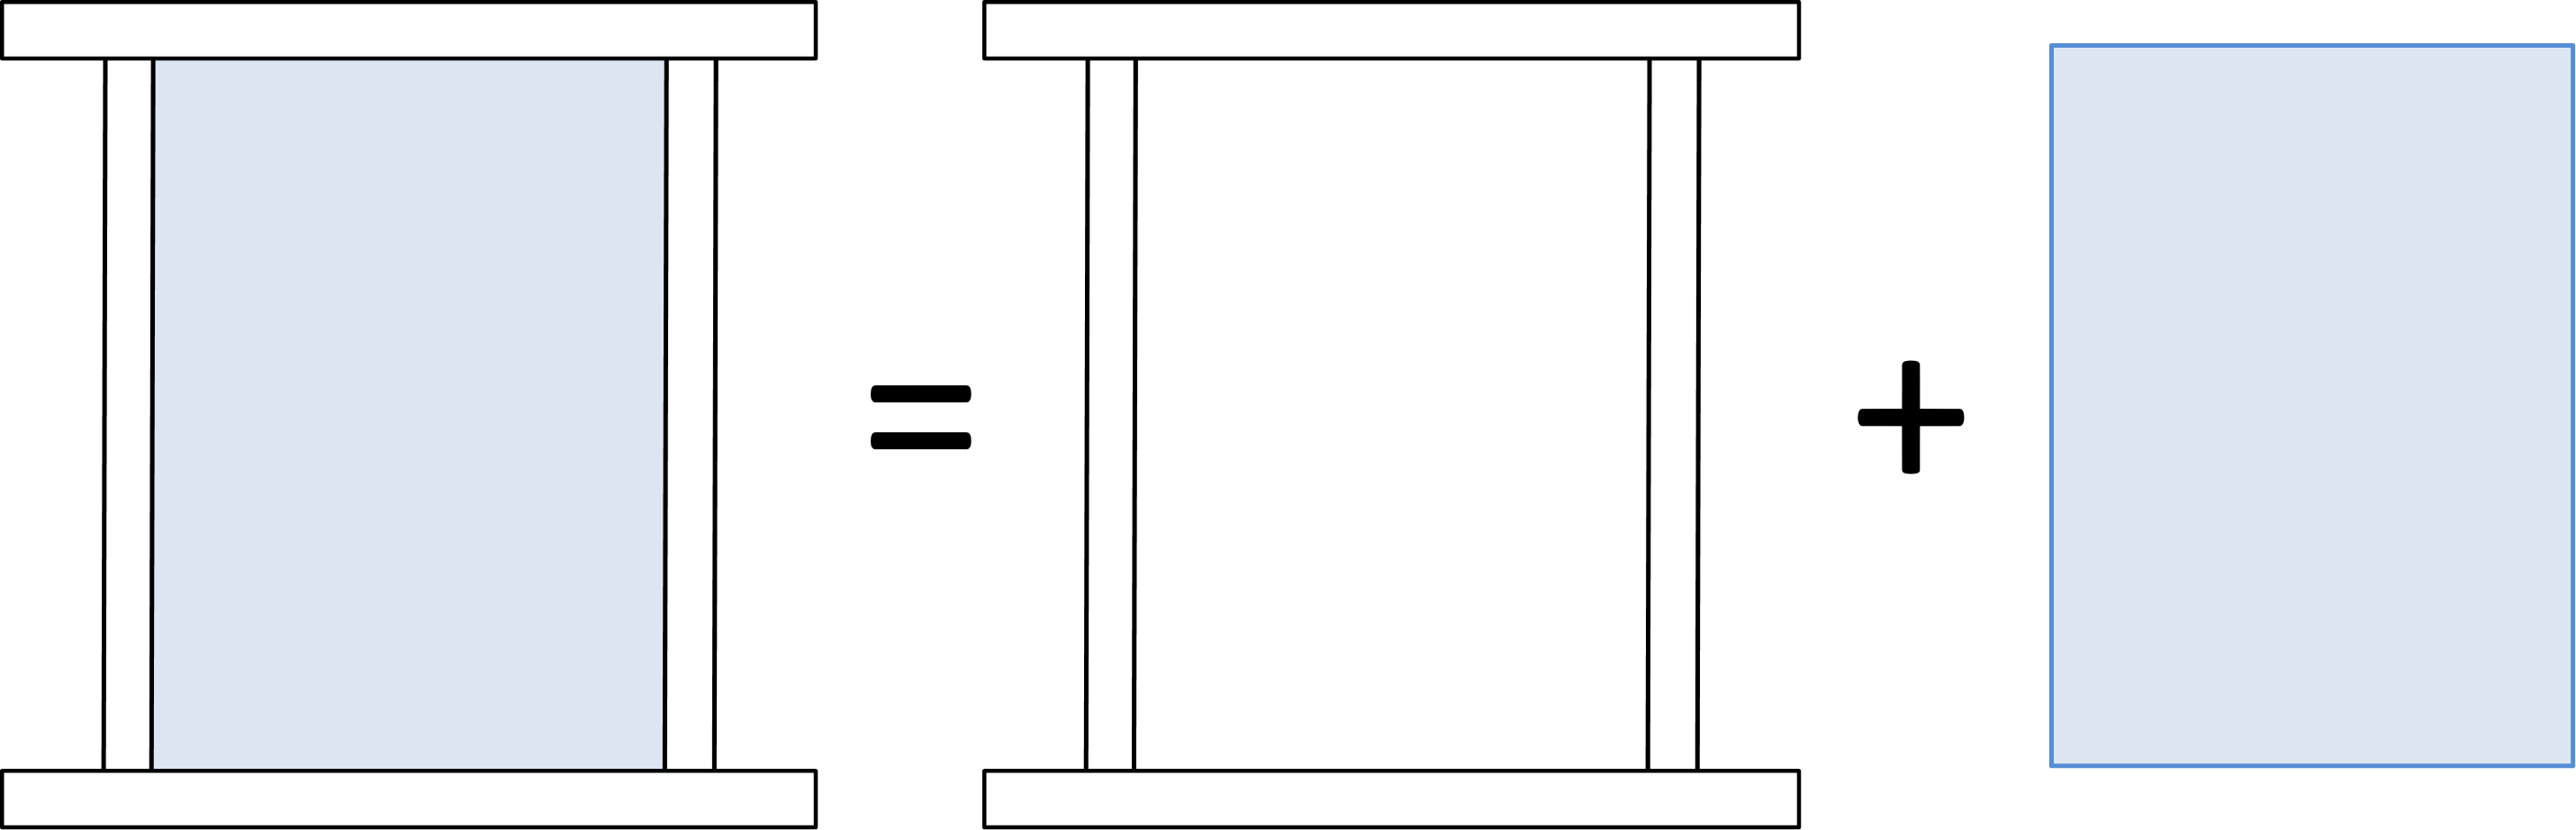
\includegraphics[width=\textwidth]{fig1}
\caption{土塗り全面壁$Q=$軸組$Q_f+$土壁パネル$Q_w$}
\label{fig:1}
\end{minipage}\hfill
\begin{minipage}[b]{0.45\textwidth}
\centering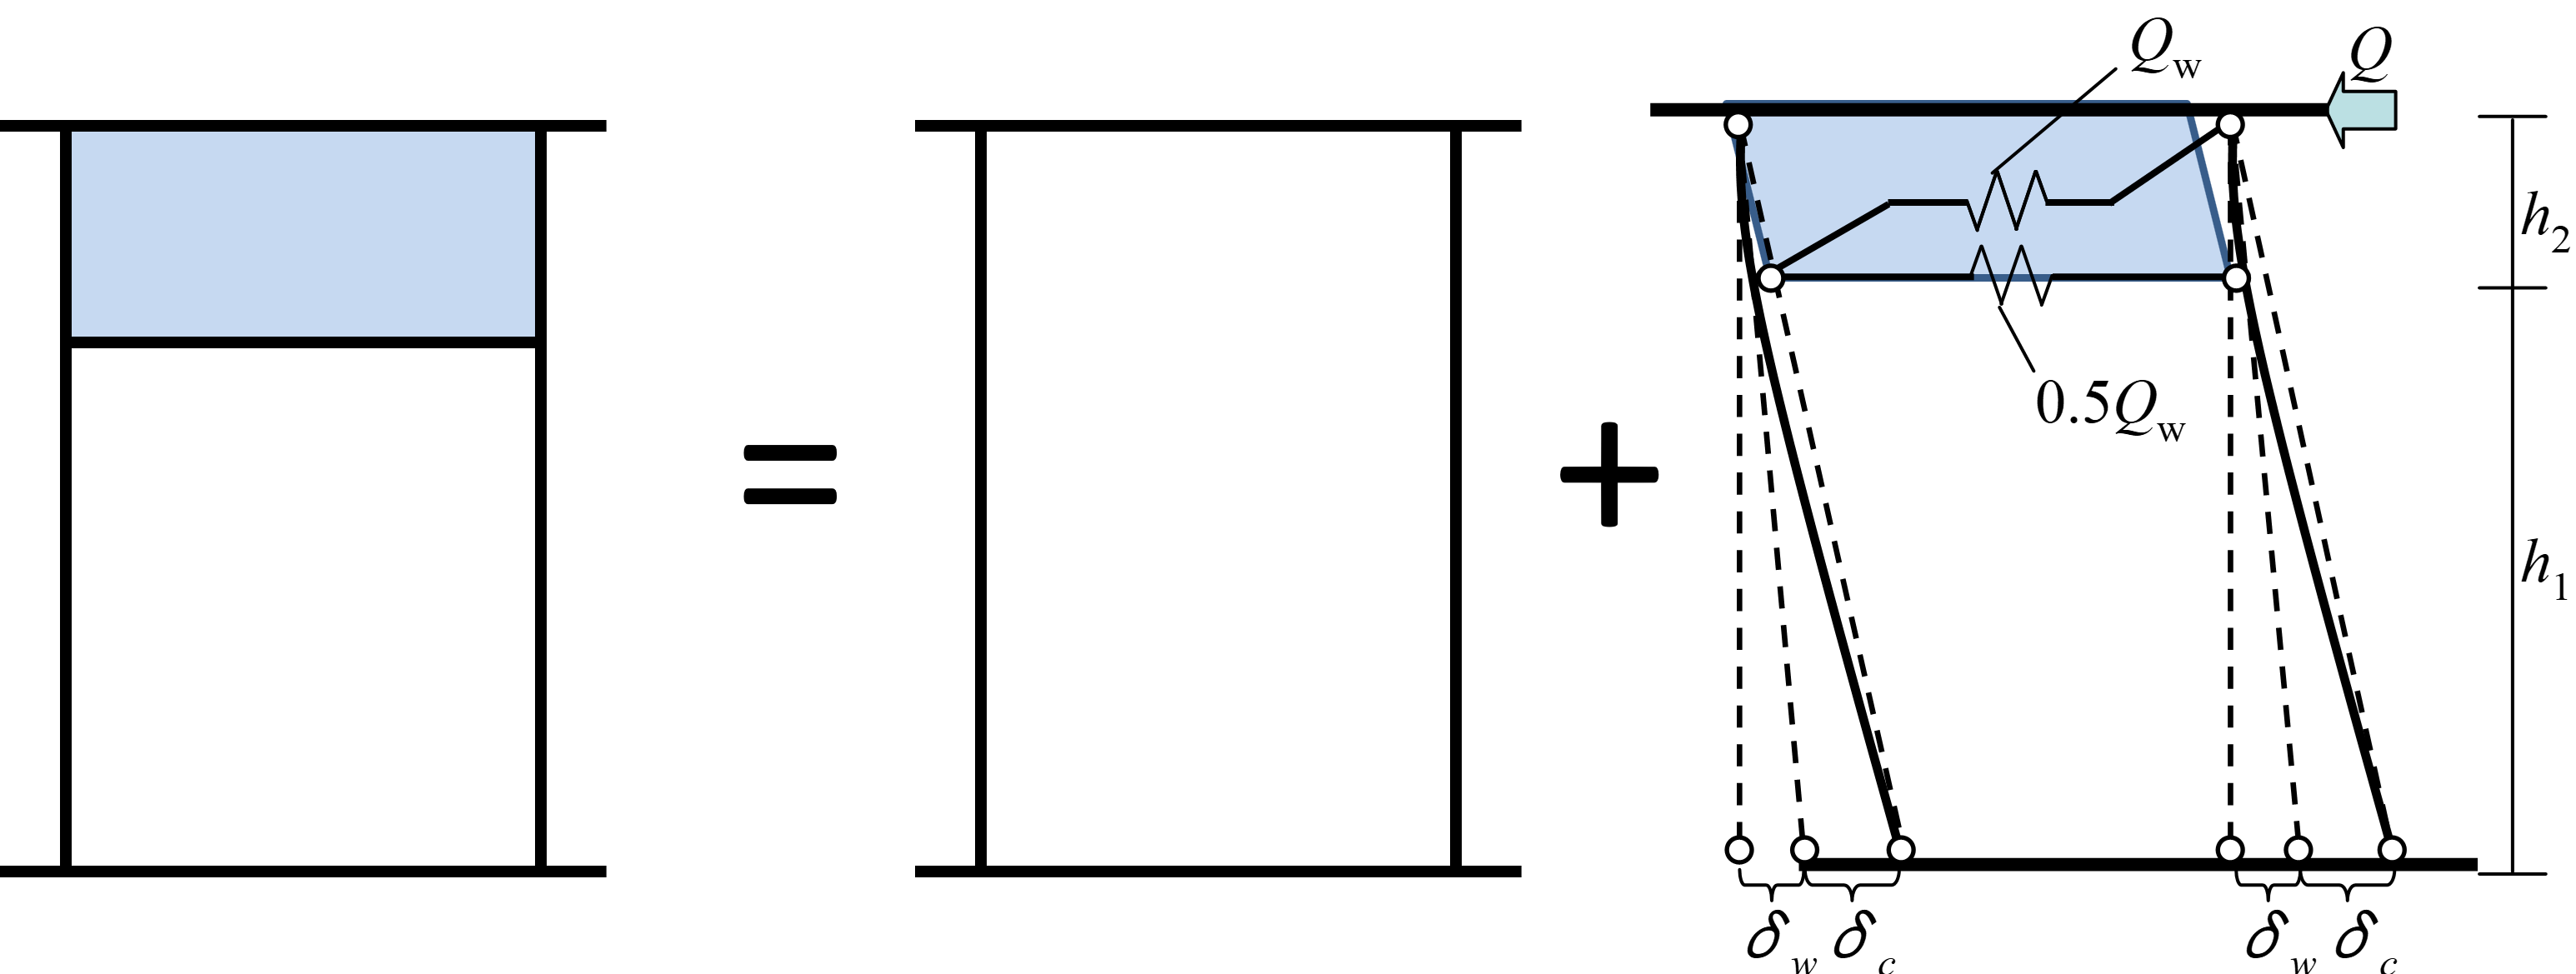
\includegraphics[width=\textwidth]{fig2}
\caption{土塗り小壁$Q=$軸組$Q_f+$軸組の曲げ変形を考慮した土壁パネル$Q_w$}
\label{fig:2}
\end{minipage}
\end{figure}
\vspace{-\baselineskip}

\paragraph{(3) 本研究の着想に至った経緯や、関連する国内外の研究動向と本研究の位置づけ}
\mbox{}\par

土塗り壁の復元力特性を精密に予想する際、上記のように軸組と土壁パネルとに分
けて考え、のちに加算する方法\cite{kentouiinkai2012,manual2019}は、構造力学
で「重ね合わせの原理」として用いられる方法である。一
方、木材や壁土等の材料強度や構造部材の接合 (継手・仕口) の力学特性からこれ
らを予想する方法は、伝統的構法に限らず木質構造全般でも未だ構築途上であ
る\cite{miyamoto2015}ため、現時点では、実大実験も併せて行うことが必須である。

応募者が土塗り壁の耐震性能に関する研究に着手した当時、日本国内では木構造(木
質構造)に関する研究は下火であり、阪神・淡路大震災の経験からその分野の研究の
重要性が見直されようとしている頃であった。土塗り壁の耐震性能を再検
討\cite{tuchikabe1999}した結果、土塗り壁の復元力特性には、貫等の下地を含ん
だ土壁パネルの復元力$Q_w$とその周囲を囲む木造軸組の復元力$Q_f$が支配的と考
えられたが、同時に、$Q_w$だけを実大実験で得ることが、難しいけれども、重要で
あることも明らかになった。このようなことから、長年、土壁パネルのみの復元
力($Q_w$)を得ることの重要性を感じてきたが、これまでは、軸組を含めた様々なサ
イズや小壁パターンでの復元力($Q$)を求めるための実大実験を優先的に続けてきた。
土壁を施工しない軸組だけの実験($Q_f$が得られる)は比較的容易であるため、$Q_w=Q-Q_f$と
仮定して、マニュアル\cite{manual2019}ではなるべく簡便に計算できるように構成
されたので、はたして、土壁パネルのみの復元力($Q_w$)を実大実験で得ることがで
きるとマニュアルがよりよいものになる、すなわち、学術的により適切であり実用
性が高まると考えるに至った。

実際には、$Q_w$のうち貫下地の寄与$Q_n$をすっかり無視することはできないと考
えられる。つまり、$Q=Q_w+Q_f=Q_w'+Q_n+Q_f$となる$Q_n$の寄与を無視できない場
合があるかどうかについても、本研究で明らかにしたい。

土壁パネルの製作では周囲を木造軸組で囲む必要があり、単にせん断加力を行おう
としても、軸組接合部(仕口)の回転抵抗や軸組の曲げ変形の影響を無視することが
できない。土壁パネル内の壁土のせん断強度を明らかにするために土壁パネル単体
にせん断変形を生じさせようとする実験はこれまでにも行われてい
る\cite{fukumoto2000}が、パネル形状が正方形に限られる等、試験体形状や実験方
法に改善が必要である。また、壁土のせん断強度に関して、例えば、越智らによる
検討\cite{ochi2019}があり、壁土強度と土壁の復元力$Q$の関係について、山田ら
の解析的検討\cite{yamada2011}がある他、土壁の復元力に関する研究はここ10年間
で少しずつ増えている。しかしながら、実大実験に基づいて土壁パネルのみの復元
力($Q_w$もしくは$Q_w'$)を求めるというアプローチは、実験が困難であるのか少な
いので、このような研究は意義深いものと考える。

\paragraph{(4) 本研究で何をどのように、どこまで明らかにしようとするのか}
\mbox{}\par

実大実験に基づいて土壁パネルのみの復元力($Q_w$)を求めるため、適切な試験体形
状を定める必要がある。軸組接合部(仕口)の回転抵抗がほぼ0となるよう、仕口
を鋼材を用いたピン接合として、大変形時に軸組の木材同士の接触を避けるよう、
柱端部に25 mm程度のすきまを空けることとする(図\ref{fig:3})。

\begin{figure}[htb]
  \begin{minipage}{0.6\textwidth}
    \centering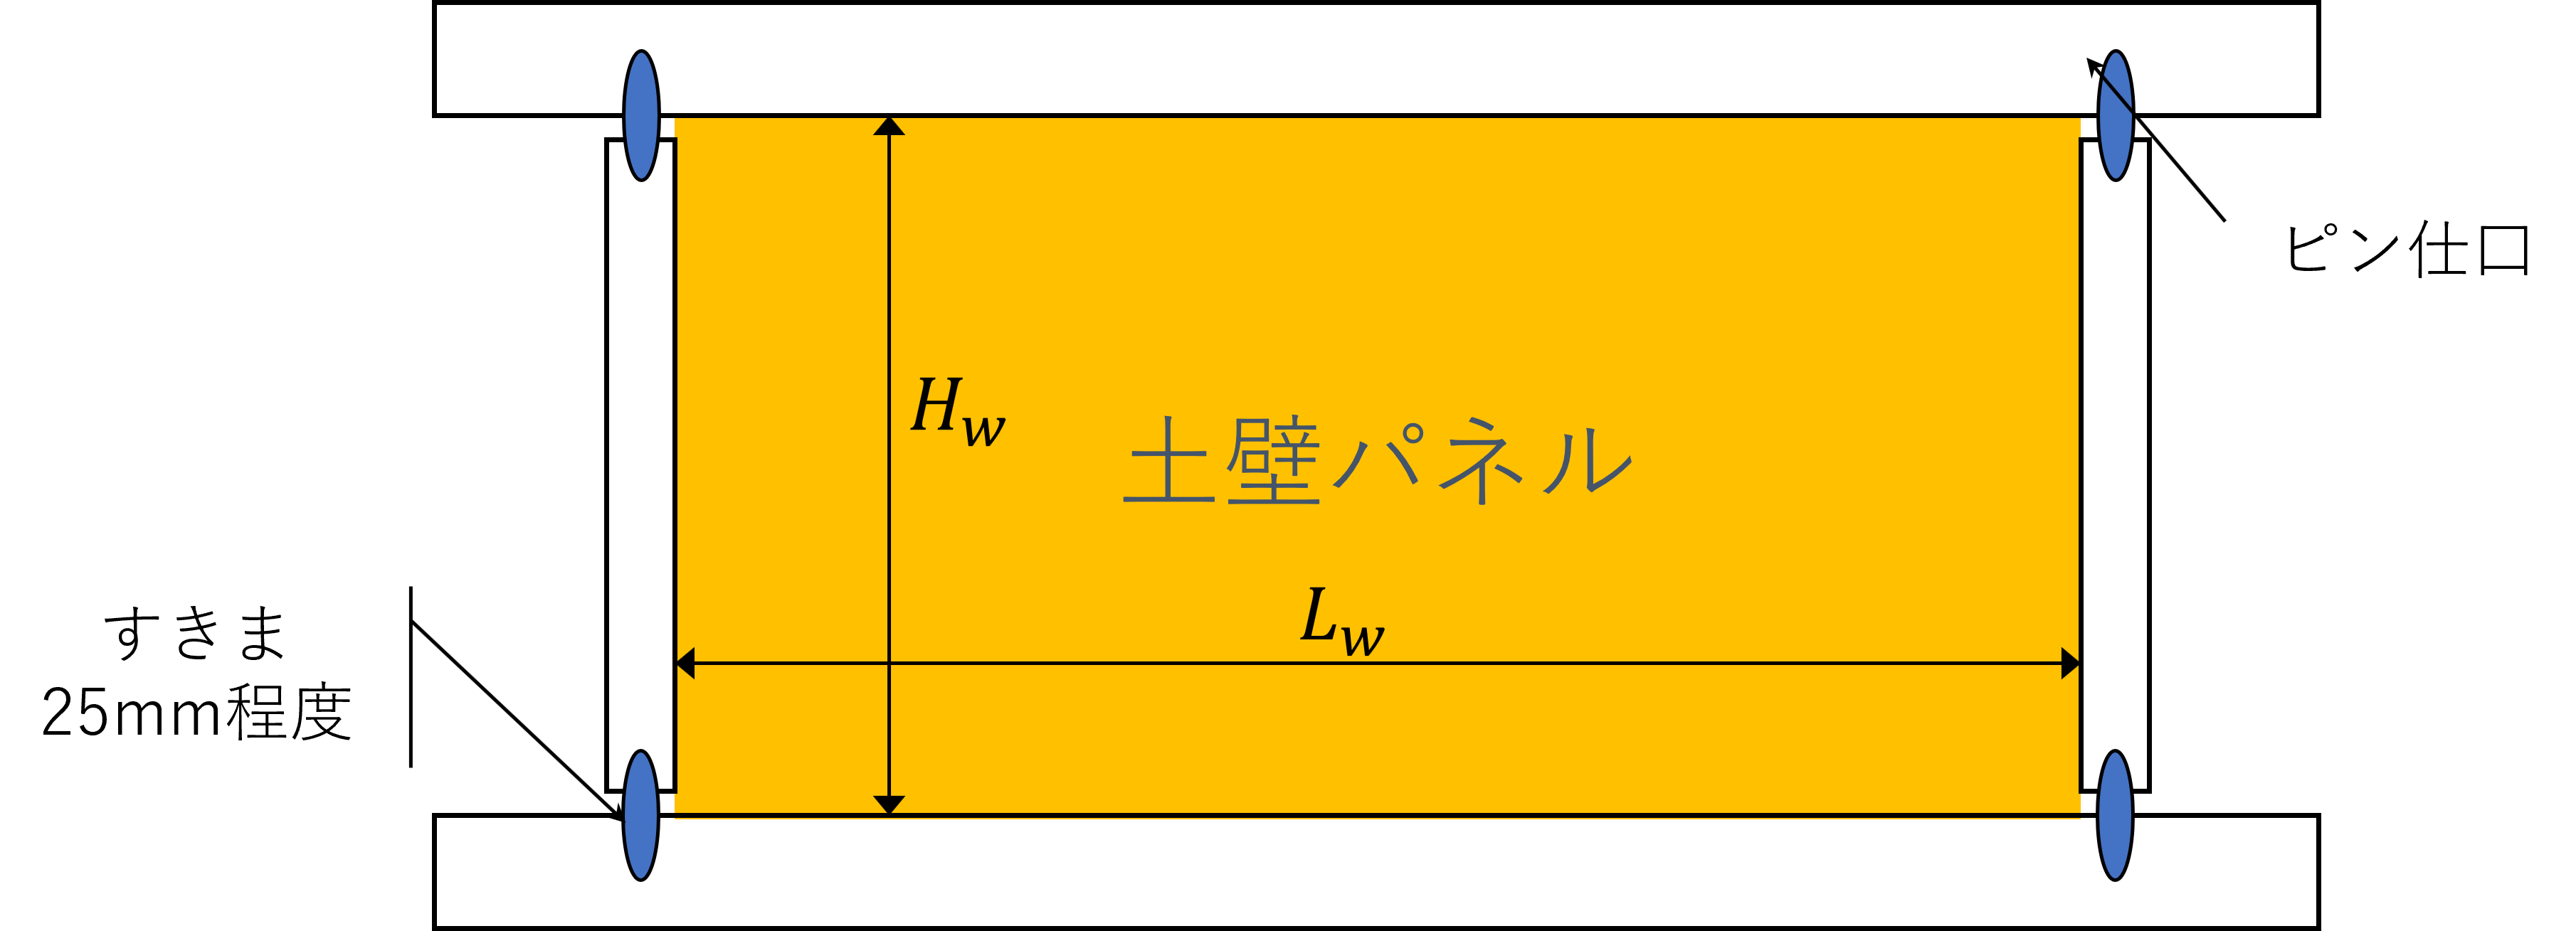
\includegraphics[width=0.95\textwidth]{fig3}
    \figcaption{試験体形状案}
    \label{fig:3}
  \end{minipage}
  \quad
  \begin{minipage}{0.35\textwidth}
    \centering
    \vspace{-1cm}
    \tblcaption{土壁パネルの試験体案 ($H_w$と$L_w$ (mm))}
    \label{tab:1}
    \begin{tabular}[htb]{|c|c|c|c|}
      \hline
      & (1) & (2) & (3)  \\\hline
      $H_w$ &  465 & 800 & 1260 \\\hline
      $L_w$ &  1700 & 790 & 790 \\\hline
    \end{tabular} 
  \end{minipage}
\end{figure}

本研究では、これまでに行った小壁付き木造軸組の実大実験結果と比較できるよう、
異なる土壁パネルサイズ($H_w$、$L_w$ (mm)の組み合わせ、表\ref{tab:1})の試験
体を各サイズについて2体ずつ製作% (試験体1つあたりおよそ60万円)
し、それぞれについて面内せん断
加力実験を行う。木造軸組だけの実験、貫下地がついた状態での実験、中塗り仕
上げまで施したものについての実験を行い、上記の復元力特性$Q$におけ
る$Q_w$、$Q_f$および$Q_n$を明らかにする。
面内せん断加力実験は、これま
で\cite{kakenhi2019}同様、桁部の水平変位を試験体高さで除した「見かけの変形
角」
が$\pm$1/480、$\pm$1/240、% $\pm$1/120、$\pm$1/90、$\pm$1/60、$\pm$1/45、
% $\pm$1/30、$\pm$1/20、$\pm$1/15
…、$\pm$1/10 radとなるように増加さ
せ、それぞれの変形を3回経験するような正負繰り返し変形制御加力とする。荷重と
各部の変形を計測する。

\一年目西暦{}年度の前半に表\ref{tab:1}の試験体(1)〜(3)を各1体製作し、
\一年目西暦{}年度後半から\二年目西暦{}年度前半にかけて、実大実験を行う。実
大実験は、大学内に既設の面内せん断実験装置を用いて行う。\二年目西暦{}年度後
半から\三年目西暦{}年度にも引き続き、必要な改善を検討した上で同様の実大実験
を行う。実験結果に基づき、マニュアルとの整合性を検証するとともに、必要に応
じて、マニュアルの改善を検討する。



\paragraph{(5) 本研究の目的を達成するための準備状況}
\mbox{}\par

1998年度から土塗り壁の耐震性能に関する実験研究
\cite{tuchikabe1999,nakajirekibo2018}を
続けており、現在の所属機関の実験設備は、土塗り壁の実大面内せ
ん断加力実験に最適化されている。変位計等一部の設備備品は当初導入から10年を
超えてメンテナンス不可となったものもあり更新の必要があるため、研究経費に含
める。\vspace{\baselineskip}

% \begin{itemize}
% \itemsep=-3pt
% \item 荷重容量が100 kNで、全振幅800 mmの電動アクチュエータによる押し引き加力が可能
% \item 高速なデータロガーによる同時80点の静ひずみ計測が可能
% \item 最大0.001 mm精度での変位計測
% \item 高速データロガーに対応した専用の計測ソフト
% \item 計測ソフトと連携して計測時の写真撮影が可能
% \end{itemize}

\renewcommand{\refname}{\textbf{参考文献}\vspace{-0.5\baselineskip}}
\begin{thebibliography}{99}
  \itemsep=0pt
  \small
\bibitem{aij1995} 日本建築学会編著: 1995年兵庫県南部地震災害調査速報,日
  本建築学会,丸善, 1995
  
\bibitem{tuchikabe1999} 鈴木祥之, 中治弘行:木造住宅土塗り壁の実大実験による耐震性能の再検討
  ,日本建築学会構造系論文集 64(515), pp.115-122, 1999
  
\bibitem{murakami2005} 例えば、村上 雅英, 景山 誠, 岡本 滋史, 鈴木 有, 稲
  山 正弘: 要素試験による土壁の水平力耐荷機構の検証 : せん断破壊が先行し
  ない土壁の力学挙動(続), 日本建築学会構造系論文集, 70 巻, 594 号,
  pp. 111-118, 2005
  
\bibitem{sympo2001} 日本建築学会近畿支部・日本建築学会「木構造と木造文化の
  再構築」特別研究委員会: シンポジウム 木構造と木造文化の再構築, 2001
  
\bibitem{kitahara2002} 北原 昭男, 林 康裕, 奥田 辰雄, 鈴木 祥之, 後藤 正美:
  2000年鳥取県西部地震における木造建物の構造特性と被害, 日本建築学会構造系
  論文集, 67 巻, 561 号, pp. 161-167, 2002
  
\bibitem{kentouiinkai} 「伝統的構法の設計法作成及び性能検証実験」検討委員会.\\
  \url{http://green-arch.or.jp/dentoh/index.html}
  
\bibitem{kentouiinkai2012} 「伝統的構法の設計法作成及び性能検証実験」検討
  委員会:詳細設計法(案)ほか,2014年
  
\bibitem{manual2019} 伝統的構法木造建築物設計マニュアル編集委員会:伝統的
  構法のための木造耐震設計法 石場建てを含む木造建築物の耐震設計・耐震補強
  マニュアル,学芸出版社,2019
  
\bibitem{kyoyououryoku2017} 木造軸組工法住宅の許容応力度設計 (2017年版),
  公益財団法人日本住宅・木材技術センター, 2017
  
\bibitem{fukumoto2000} 福本和正:壁土のせん断強度の実験的研究,日本建築学
  会構造系論文集(530) pp.99-06,2000
  
\bibitem{ochi2019}  越智隆行, 宮本慎宏, 宇都宮直樹, 松島学:原位置採取試料
  による壁土の強度特性評価手法の提案.日本建築学会技術報告集 (59),
  pp.45-50, 2019
  
\bibitem{yamada2011} 山田 耕司, 中治 弘行, 鈴木 祥之:異なる強度を持つ壁土
  を用いた土壁耐力の推定.日本建築学会構造系論文集 76(660), pp.347-352,
  2011
  
\bibitem{miyamoto2015} 例えば、宮本慎宏他: 開口部を有する土塗壁の耐力変形
  角推定式の提案,構造III (2015), 日本建築学会, pp.313-316, 2015
  		
\bibitem{kakenhi2019} 例えば、束で分割された土塗り小壁付木造軸組の復元力特
  性の実大実験による検証,基盤研究(C)19K04692,研究代表者:中治弘行
  
% \bibitem{yamada-nakaji2017} 山田耕司, 中治弘行, 長瀬正, 鈴木祥之: 伝統構法木造
%   軸組における土塗り小壁の復元力評価法. 歴史都市防災論文集Vol.11,
%   pp.95-102, 2017.

% \bibitem{nakajirekibo2017} 中治弘行, 長瀬正, 山田耕司, 鈴木祥之: 実大実験に
%   基づく土塗り小壁付木造軸組の復元力特性. 歴史都市防災論文集Vol.11,
%   pp.103-110, 2017.
             
  
\bibitem{nakajirekibo2018} 中治弘行, 鈴木祥之, 長瀬正: 垂れ壁と腰壁で分割さ
  れた無開口土塗り壁の復元力特性. 歴史都市防災論文集 Vol.12, pp.23-30,
  2018.
\end{thebibliography}
%end 研究目的と研究計画 ====================

% p01_purpose_plan_01.tex
\KLEndSubject{F}


%#Split: 03_abilities  
%#PieceName: p03_abilities
% p03_abilities_00.tex
\KLBeginSubject{02}{2}{2 応募者の研究遂行能力及び研究環境}{2}{F}{}{jsps-subject-header}{jsps-default-header}

\section{2 応募者の研究遂行能力及び研究環境}
%    <<最大 2ページ>>

% s14_abilities
% \PapersInstructions		% <-- 留意事項。これは消すか、コメントアウトしてください。
%begin 応募者の研究遂行能力及び研究環境 ====================
\paragraph{(1) これまでの研究活動}
\mbox{}\par

\begin{wrapfigure}[10]{r}{7cm}
  \centering
  \vskip-1em
  \setlength{\abovecaptionskip}{1pt}
  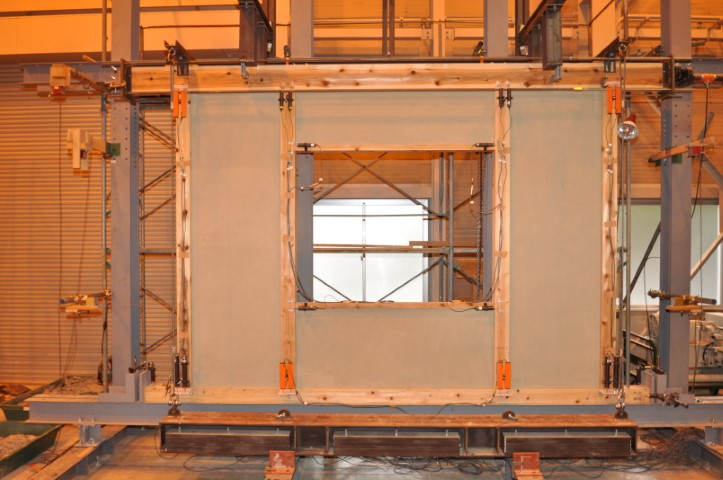
\includegraphics[width=65mm]{20110301101055_MAN}
  \caption{土塗り壁の面内せん断加力試験例}
  \label{fig:equipment}  
\end{wrapfigure}
%%%
応募者は、主に土塗り壁を対象として、図\ref{fig:equipment}に示す実験装置を用
いた面内せん断加力実験に基づく構造性能評価に関する研究を継続してい
る。2006年に現所属機関に着任以降は、鳥取県内の伝統的構法に関わる設計者や大
工、左官の人脈を広げ、実験に必要な試験体製作を依頼しやすいほか、加力や測定
器設置に必要な治具類も入手しやすい状況にある。

2010年度以降は、先述の検討委員会に参画したことにより、必要な設備が一通り
揃い、発表論文も下記に挙げるように一定数ある。また、関連テーマでの科研費あ
るいは受託研究等での外部資金獲得実績も数件ある。
\vspace{0.5\baselineskip}

%end 応募者の研究遂行能力及び研究環境 ====================
%begin 研究業績リスト ====================
{\parindent=0pt
  \textbf{<主な発表論文>}}
\vspace{-1ex}

\begin{enumerate}
  \small
  \itemsep=-2pt
% \item \label{pub:aij1999} 
%   鈴木祥之, \私{}: 木造住宅土塗り壁の実大実験による耐震性能の再検討, 日本
%   建築学会構造系論文報告集, 第515号, pp.115-122, 1999. % (査読あり)

% \item \label{pub:wcte2006} {Nakaji, H.}, Suzuki, Y., Gotou, M. and
%   Iwamoto, I: Seismic performance evaluation of traditional wooden house
%   by alternate cyclic loading test, WCTE 2006 - 9th World Conference on
%   Timber Engineering, August 2006.
%   % (査読あり)
  
% \item \label{pub:aij2007-11}
%   山田耕司, 清水秀丸, {\私{}}, 鈴木祥之:
%   土塗り小壁付木造軸組耐力特性評価への数値解析の適用,
%   日本建築学会構造系論文集、No.621, pp.81-87, 2007. % (査読あり)

% \item \label{pub:jees2007}
%   {\私{}}, 松本慎也, 向坊恭介, 宮本慎宏, 鈴木祥之:
%   能登半島地震における木造建物の詳細調査と限界耐力計算結果,
%   日本地震工学会第5回年次大会, pp.428-429, 2007. % (査読あり)

% \item \label{pub:aij2007-mikawa}
%   {\私{}}, 鈴木祥之, 後藤正美, 岩本いづみ, 山田耕司:
%   東三河伝統構法民家の耐震性能評価のための静的繰り返し加力実験,
%   日本建築学会構造系論文集, No.612, pp.133-140, 2007. % (査読あり)

\item \label{pub:wcte2008}
  \me{}, Koji Yamada, Tatsuru Suda and   Yoshiyuki Suzuki:
  Seismic Performance Verification of
  Traditional Wooden House Based on Cyclic Loading Tests and
  Analytical Methods,
  WCTE 2008 - 10th World
  Conference on Timber Engineering, pp.1866-1873, 2008. % (査読あり)


\item \label{pub:jees2010}
  \私{}, 山田耕司, 鈴木祥之:
  鳥取県の工法による土塗り壁を有する木造軸組架構の耐力特性評価,
  第13回日本地震工学シンポジウム論文集, pp.4075-4078, 2010. % (査読あり)

\item \label{pub:wcte2010}
  \me{}, Koji Yamada, Masato Nakao, Yoshiyuki Suzuki: 
  SEISMIC CAPACITY EVALUATION OF MUD-PLASTERED
  WALLS CONSIDERING STRENGTH OF MUD, 
  WCTE 2010 - 11th World
  Conference on Timber Engineering, pp.2201-2206, 2010. % (査読あり)


\item \label{pub:wcte2012}
  \me{}, Teruo Kamada, Masami Gotou, Koji Yamada,
  Yoshiyuki Suzuki:
  SEISMIC PERFORMANCE OF MUD-WALLS WITH SILL BASED ON FULL-SCALE
  CYCLIC LOADING TESTS,
  World Conference on Timber Engineering 2012, pp.456-459, 2012. % (査読あり)


\item \label{pub:wcte2014} \me{}, Masami Gotou, Hiro Kawahara, Yoshiyuki
  Suzuki: EVALUATION OF RESTORING FORCE CHARACTERISTICS OF MUD-WALLS
  CONSIDERING EFFECT OF WALL-HEIGHT FOR SEISMIC STRUCTURAL DESIGN, World
  Conference on Timber Engineering 2014, USB stick (ページ記載なし),
  2014. % (査読あり)

% \item \label{pub:rekibo2015} 
%   \私{}, 鈴木祥之:
%   顕しの貫がある土壁の復元力特性, 
%   歴史都市防災論文集Vol.9, pp.109-114, 2015. % (査読あり)

\item \label{pub:wcte2016} 
  \me{}, Yoshiyuki Suzuki:
  Influence of Penetrating Tie Beams Visible from the Front of
  Wall on Restoring Force Characteristics of Mud-Walls,
  World Conference on Timber Engineering 2016, pp.5439-5446, 2016. % (査読あり)


\item \label{pub:rekibo2017-yamada} 山田耕司, \私{}, 長瀬正, 鈴木祥之: 伝
  統構法木造軸組における土塗り小壁の復元力評価法. 歴史都市防災論文集
  Vol.11, pp.95-102, 2017. % (査読あり)
  
\item \label{pub:rekibo2017-nakaji} \私{}, 長瀬正, 山田耕司, 鈴木祥之: 実
  大実験に基づく土塗り小壁付木造軸組の復元力特性. 歴史都市防災論文集
  Vol.11, pp.103-110, 2017. % (査読あり)
  
\item \label{pub:rekibo2018-nakaji} \私{}, 鈴木祥之, 長瀬正: 垂れ壁と腰壁
  で分割された無開口土塗り壁の復元力特性. 歴史都市防災論文集 Vol.12,
  pp.23-30, 2018. % (査読あり)

	\end{enumerate}
%end 研究業績リスト ====================
{\parindent=0pt
  \textbf{<これまでに受けた研究費等>}}

現在の所属機関に着任後に受けた競争的資金等のうち本研究と関連の深いものは
以下のとおりである。

\begin{itemize}
  \small
  \itemsep=-2pt
\item 基盤研究(S) (一般)、2007--2011年度、
  「伝統木造建築物の構造ディテールに基づく設計法の構
  築に関する研究(鈴木祥之)」、課題番号19106010、
  研究分担者、\Number{7600}千円

\item 若手研究(B)、2008--2009年度、
  「土塗り壁を有する木造軸組架構の耐力特性評価実験」、
  課題番号20760381、
  研究代表者、\Number{3300}千円

\item 基盤研究(C) (一般)、2008--2010年度、
  「土壁ラーメン架構耐力特性の解明(山田耕司)」、
  課題番号20560542、
  研究分担者、\Number{2800}千円

\item 基盤研究(C) (一般)、2011--2013年度、
  「伝統大工技術により補修された木造軸組架構の性能評価実験」、
  課題番号23560685、
  研究代表者、\Number{4200}千円

\item 受託研究 (NPO法人緑の列島ネットワーク)、2010年度、
  「伝統的構造要素としての土塗り壁の実大実験」、
  研究代表者、\Number{3000}千円

\item 受託研究 (NPO法人緑の列島ネットワーク)、2011年度、
  「土壁用軸組の復元力特性の検出」、
  研究代表者、\Number{500}千円

\item 受託研究 (NPO法人緑の列島ネットワーク)、2012年度、
  「高さの異なる土台仕様土塗り壁の力学特性評価実験」、
  研究代表者、\Number{400}千円

\item 研究助成 (公益財団法人 松井角平記念財団)、2016年度、
  「山陰地方の大規模木造建物における土塗り小壁付大断面木造軸組の
  耐震性能評価実験」、研究代表者、\Number{1200}千円
  
  \item 基盤研究(C)(一般)、2019-2021年度、「束で分割された土塗り小壁付木造
    軸組の復元力特性の実大実験による検証」、課題番号19K04692、研究代表者、
    \Number{4420}千円
    
\end{itemize}


\paragraph{(2) 研究環境}
\mbox{}\par

所属機関の実験設備は、準備状況でも述べたように、土塗り壁の実大面内せん断加
力実験に最適化されており、応募者が専有できる状態である。実験に使用できる主
な設備備品等は以下の通りである。

\begin{itemize}
\itemsep=-2pt
\item 木造耐力壁の面内せん断加力装置 (反力壁、反力床含む)
\item 高速データロガー TDS-530,(株)東京測器研究所
\item スイッチボックス IWH-50G,(株)東京測器研究所
\item 計測ソフト TDS-7130v2 (公立鳥取環境大学仕様),(株)東京測器研究所
\item 電動アクチュエータ AE80,THK(株)
\item 万能試験機 UH-1000kNI,(株)島津製作所
\item 荷重計 TCLP-30KNB・TCLP-50KNB・TCLP-100KNB (各1台),(株)東京測器研究所
\item 変位計 CDP-50 (12台)・CDP-100 (10台)・SDP-100 (8台)他,(株)東京測器研究所
\item デジタルカメラ D7500,(株)ニコン
\item など
\end{itemize}

その他、研究資料の入手については、日本建築学会のデータベースやCiNii等のイン
ターネットを活用した方法のほか、所属機関の図書館を中心として書籍等の閲覧が
可能である。実験の準備や実施においては、実験手法の教育を兼ねて、学部学生や
大学院生の手腕を頼ることができる体制を整えている。

% p03_abilities_01.tex
\KLEndSubject{F}


%#Split: 04_rights  
%#PieceName: p04_rights
% p04_rights_00.tex
\KLBeginSubject{03}{3}{3 人権の保護及び法令等の遵守への対応}{1}{F}{}{jsps-subject-header}{jsps-default-header}

\section{3 人権の保護及び法令等の遵守への対応}
%    <<最大 1ページ>>

% s09_rights
%begin 人権の保護及び法令等の遵守への対応 ====================
研究計画を遂行するに当たって、相手方の同意・協力を必要とする研究、個人情報
の取り扱いの配慮を必要とする研究、生命倫理・安全対策に対する取組を必要とす
る研究など法令等に基づく手続が必要な研究には該当しない。
%end 人権の保護及び法令等の遵守への対応 ====================

% p04_rights_01.tex
\KLEndSubject{F}


%#Split: 05_final_year  
%#PieceName: p05_final_year
% p05_final_year_00.tex
\KLBeginSubject{04}{4}{4 研究計画最終年度前年度応募を行う場合の記述事項}{1}{F}{}{jsps-subject-header}{jsps-default-header}

\section{4 研究計画最終年度前年度応募を行う場合の記述事項}
%    <<最大 1ページ>>

%s04_prep_finalyear
% 2020-08-16: Taku: Adjusted the horizontal position of the tabular.
%begin 最終年度の研究課題 ====================
\newcommand{\最終年度研究種目名}{\quad{}}
\newcommand{\最終年度研究課題番号}{\quad{}}
\newcommand{\最終年度研究課題名}{\quad{}}
\newcommand{\最終年度研究期間}{令和\quad{}年度〜令和\一年目 年度}
%end 最終年度の研究課題 ====================
% p05_final_year_01.tex
\noindent
\hspace{-7pt}
\begin{tabular}{|p{118pt}|p{44pt}|p{208pt}|p{46pt}|}
	\hline
	\KLTabC{\textbf{研究種目名}} & 
	\KLTabC{\textbf{課題番号}} & 
	\KLTabC{\textbf{研究課題名}} & 
	\KLTabC{\textbf{研究期間}}\\
	\hline
	\最終年度研究種目名 &
	\最終年度研究課題番号 &
	\最終年度研究課題名 &
	\最終年度研究期間 \\
	\hline
\end{tabular}
\\


\noindent
\textbf{当初研究計画及び研究成果}\\
%begin 研究計画最終年度の応募の計画と成果 ====================

%end 研究計画最終年度の応募の計画と成果 ====================
% \\

\noindent
\textbf{前年度応募する理由}\\
%begin 研究計画最終年度の応募の理由 ====================

%end 研究計画最終年度の応募の理由 ====================

% p05_final_year_02.tex
\KLEndSubject{F}


%#Split: 99_tail
% hook9 : right before \end{document} ============
 % pieces
\end{document}

